\documentclass[]{beamer}
\usetheme[secheader]{Boadilla}

\mode<presentation>{}

\usepackage{boxedminipage}

\newcommand{\prob}[1]{{\rm Prob}\left[#1\right]}
\newcommand{\secprm}{\lambda}
\newcommand{\zu}{\{0,1\}}
\newcommand{\from}{\leftarrow}
\newcommand{\negl}{{\mathsf{negl}}}
\newcommand{\poly}{{\mathsf{poly}}}
\newcommand{\aux}{{\mathsf{aux}}}

\newcommand{\calD}{\mathcal{D}}    %the dictator
\newcommand{\calE}{\mathcal{E}}    %encryption scheme
\newcommand{\calF}{\mathcal{F}}    %PRF

\newcommand{\algofont}[1]{{\mathsf{#1}}}
\newcommand{\gamefont}[1]{{\mathsf{#1}}}
\newcommand{\objfont}[1]{{\mathtt{#1}}}



%the normal triplet
\newcommand{\kg}{\algofont{KG}}
\newcommand{\enc}{\algofont{Enc}}
\newcommand{\dec}{\algofont{Dec}}
%the anamorphic triplet
\newcommand{\akg}{\algofont{a}\kg}
\newcommand{\aenc}{\algofont{a}\enc}
\newcommand{\adec}{\algofont{a}\dec}

\newcommand{\constr}{\algofont{AME}}

%Goldwasser Micali
\newcommand{\GM}{\algofont{GM}}

%Naor Yung
\newcommand{\ny}{\algofont{ny}}
\newcommand{\nye}{\ny\algofont{E}}

%koppula waters
\newcommand{\kw}{\algofont{kw.}}
\newcommand{\kwkg}{\kw\kg}
\newcommand{\kwenc}{\kw\enc}
\newcommand{\kwdec}{\kw\dec}
\newcommand{\signk}{\objfont{sigK}}
\newcommand{\verk}{\objfont{vK}}
\newcommand{\signature}{\algofont{Sign.}\kg}


\newcommand{\ct}{\objfont{ct}}      %ciphertext
\newcommand{\pk}{\objfont{PK}}      %public key
\newcommand{\fpk}{\objfont{f}\pk}   %the forced public key
\newcommand{\dpk}{\objfont{d}\pk}   %the duplicate public key
\newcommand{\sk}{\objfont{sk}}      %secret key
\newcommand{\fsk}{\objfont{f}\sk}   %the forced secret key
\newcommand{\dsk}{\objfont{d}\sk}   %the duplicate secret key

\newcommand{\apk}{\objfont{a}\pk}   %anamorphic public key
\newcommand{\ask}{\objfont{a}\sk}   %anamorphic secret key
\newcommand{\act}{\objfont{a}\ct}   %anamorphic ciphertext
\newcommand{\dkey}{\objfont{dkey}}  %double key
\newcommand{\fct}{\act}             %deprecated


%games
\newcommand{\NormalG}{\gamefont{NormalG}}
\newcommand{\FullyAG}{\gamefont{FullyAG}}


%signature schemes
\newcommand{\signatureSchemeName}{\algofont{S}}
\newcommand{\signPrefix}{\algofont{}}
\newcommand{\signkg}{\signPrefix\kg}
\newcommand{\pseudogen}{\signPrefix\algofont{PG}}
\newcommand{\signsign}{\signPrefix\algofont{Sig}}
\newcommand{\signverify}{\signPrefix\algofont{Verify}}
\newcommand{\accept}{\mathtt{Accept}}
%objects for signatures
\newcommand{\signOPrefix}{\objfont{s}}
\newcommand{\svk}{\signOPrefix\objfont{vk}}
\newcommand{\ssk}{\signOPrefix\objfont{sk}}
\newcommand{\ssignature}{\objfont{sig}}
\renewcommand{\ssignature}{\Sigma}
%game for signature
\newcommand{\sigGame}{\gamefont{sigG}}
\newcommand{\osig}{\oracle\algofont{s}}
\usepackage{tikz}
\usepackage{tikzpeople}
\newcommand{\msg}{{\mathtt{msg}}}
\newcommand{\amsg}{{\mathtt{amsg}}}


\newcommand{\anamorphicPrefix}{\algofont{a}}
\newcommand{\anamorphicPrefixObj}{\objfont{a}}
\newcommand{\ame}{\algofont{AME}}
%\newcommand{\adec}{\anamorphicPrefix\dec}
%\newcommand{\apk}{\anamorphicPrefixObj\pk}
%\newcommand{\ask}{\anamorphicPrefixObj\sk}
%\newcommand{\dkey}{\objfont{dkey}}
\newcommand{\rdkey}{\objfont{rdk}} %receiver double key
\newcommand{\sdkey}{\objfont{sdk}} %sender/signer double key
\newcommand{\vdkey}{\objfont{vdk}} %verifier double key
%\newcommand{\act}{\anamorphicPrefixObj\ct}
%\newcommand{\amsg}{\anamorphicPrefixObj\msg}

\newcommand{\at}{\algofont{T}} %the anamorphic triplet

%%anamorphic signatures
\newcommand{\asignkg}{\anamorphicPrefix\signkg}
\newcommand{\dkg}{\mathsf{d}\signkg}
\newcommand{\asignsign}{\anamorphicPrefix\signsign}
\newcommand{\dsigGame}{\gamefont{DsigG}}
%%objects
\newcommand{\asvk}{\anamorphicPrefixObj\svk}
\newcommand{\assk}{\anamorphicPrefixObj\ssk}
\newcommand{\assignature}{\anamorphicPrefixObj\ssignature} %anamorphic signature
%%
\newcommand{\extr}{\algofont{Extract}}


\usetikzlibrary{snakes}
\usetikzlibrary{backgrounds} 
\usepgflibrary{shapes.geometric}
\usepgflibrary{shapes.misc}
\usetikzlibrary{shapes.callouts}
\usetikzlibrary{bending}
\usepackage{pgfmath}


\title[Anamorphic]{Anamorphic Cryptography: Current Developments}
\subtitle{Private Communication against a Dictator}
\author{Giuseppe Persiano}

\date{Summer School on Real-World Crypto and Privacy -- June 2024}

\begin{document}

\begin{frame}
  \titlepage



Joint work with:

{Duong Hieu Phan, Moti Yung}
and
Miroslaw Kutylowski, Marcin Zawada. 

\end{frame}


\begin{frame}

\frametitle{Content}

\begin{itemize}
\item Receiver-Privacy and Sender-Freedom: Dictators and Crypto Wars
\item Our Approach for Receiver-Privacy: No New Constructions
\item Receiver-Privacy: Formal Definitions 
\item Receiver-Privacy: Constructions
    \begin{itemize}
        \item General result with low rate
        \item Randomness Recoverable Encryption
        \item CCA secure Encryption
    \end{itemize}
\item Signatures
\end{itemize}

\vfill
\color{brown}
Eurocrypt 2022
{\tt\color{blue}  https://ia.cr/2022/639}

PETS 2023
{\tt\color{blue}  https://ia.cr/2023/434}

Crypto 2023
{\tt\color{blue}  https://ia.cr/2023/356}

Crypto 2024

\end{frame}



\begin{frame}
\frametitle{Privacy as a Human Right}

UDHR, Article 12: (1948)

{\color{brown}
{\em No one shall be subjected to arbitrary interference with his privacy, family, home or \bf correspondence},...
}

\pause
\vskip 1cm
\begin{block}{End to End Encryption}
\begin{itemize}
\item Cryptography has been very successful in providing tools for
encrypting communication
\begin{itemize}
\item The Signal protocol and app \hfill \includegraphics[width=.5cm]{imgs/signal}
\end{itemize}
\end{itemize}
\end{block}

\pause
\vfill
But its success relies on two assumptions that might be challenged in dictatorial
states
\end{frame}

\begin{frame}
\frametitle{The receiver-privacy assumption}

{\color{brown} \em 
Encryption guarantees message confidentiality only with respect to 
parties that do not have access to  the receiver's private key
}

\vfill


\begin{block}{The receiver-privacy assumption}
The receiver keeps his secret key in a private location
\end{block}

\end{frame}

\begin{frame}
\frametitle{The sender-freedom assumption}

{\color{brown} \em 
A ciphertext carries the message that was provided as an input,
not the one that the sender wishes to encrypt
}

\vfill

\begin{block}{The sender-freedom assumption}
The sender is free to pick the message to be encrypted
\end{block}
\end{frame}

\begin{frame}
\frametitle{Receiver privacy and Sender freedom}
\begin{itemize}
\item Both assumptions are realistic for {\color{purple} ``normal''} settings
\item No wonder Encryption has been developed under these assumptions
\begin{itemize}
\item with no explicit mention
\end{itemize}
\pause
\vskip .5cm
\item In a dictatorship, instead
\pause
\begin{itemize}
\item {\color{blue} No receiver privacy:} 
citizens might be invited to surrender their private keys

\centerline{\includegraphics[width=4.1cm]{imgs/xkcd}}

\item {\color{blue} No sender freedom:} 
citizens might be invited to send messages to international newspapers
to make the dictator look good
\end{itemize}
\end{itemize}
\end{frame}

\begin{frame}
\frametitle{OK...two more assumptions}

Why is this a problem?

\begin{theorem}
Assume 
{\color{brown} existence of one-way functions} 
and 
{\color{brown} receiver privacy}.
Then, there exist secure symmetric encryption schemes.
\end{theorem}

\vfill
\begin{block}{Two assumptions}
\begin{itemize}
\item Existence of one-way functions
\item Ability to hide my key
\end{itemize}
\end{block}
\end{frame}

\begin{frame}
\frametitle{Law of Nature vs Normative Prescription}

\begin{itemize}
\item {\color{green} Assumption of the existence of one-way functions comes from
{\em our current scientific understanding of Nature}}
 
    \begin{itemize}
        \item {\color{brown}if true, it is enforced by Nature}
        \item {\color{brown}it might be false but then it is false for all}
    \end{itemize}
\vskip 1cm
\item {\color{green} Receiver privacy is a {\em norm}: }
    
    \begin{itemize}
        \item {\color{brown} it is enforced by political power}
        \item {\color{brown} it can be changed by law, decree, force}
        \item {\color{brown} it could change for some but not for all}
    \end{itemize}
\end{itemize}

\end{frame}



\begin{frame}
\frametitle{Not only dictators...}
\begin{block}{Crypto Wars}
{\em\color{brown} Presently, anyone can obtain encryption devices for voice or data transmissions. [...]
if criminals can use advanced encryption technology in
their transmissions, electronic surveillance techniques could be rendered 
useless because of law enforcement’s inability to decode the message.}

\medskip

\hfill {\color{teal} Howard S. Dakoff}

\hfill {\color{teal} {\em The Clipper Chip Proposal},}
{\color{teal} J. Marshall L. Rev., 29, 1996.}
\end{block}

\begin{block}{Ban of E2E encryption}
\color{brown}{\em
In our country, do we want to allow a means of communication between people which even in extremis, with a signed warrant from the Home Secretary personally, that we cannot read?}

\color{teal}
\hfill David Cameron

\hfill UK Prime Minister

\hfill January 2015 
%%https://www.bbc.com/news/technology-33737813
\end{block}
\end{frame}

\begin{frame}
\frametitle{Crypto Wars}

\begin{itemize}
\item Combination of cryptographic tools and normative prescription

\item From [Micali 1992] to [Green-Kaptchuk-van Laer 2021]

\begin{itemize}
\item Rely on the existence of an independent judiciary system (missing in a Dictatorship!)
\end{itemize}
\item Several related concepts
\begin{itemize}
\item Kleptography [Young-Yung 97]
\item Subvertable encryption
\item Steganography (see later)
\end{itemize}
\end{itemize}
\end{frame}

\begin{frame}
\frametitle{Crypto Wars}
Several arguments have been made against restricting encryptions:
\begin{itemize}
\color{brown}
\item {\em the bad guys can utilize other encryption systems}
\item {\em all other encryption schemes must be declared illegal}
    \begin{itemize}
        \item what qualifies as an encryption scheme? 
            e.g., {\em chaffing and winnowing}
    \end{itemize}
\item {\em it creates a natural weak systems security point}
\end{itemize}
\pause
\vskip .1cm
All these arguments are \color{red} indirect and non-technical
\pause
\vfill
\color{teal}
We wish to give technical evidence that it is {\em futile} 
    to try to restrict encryption

\centerline{\em Resistance is futile}
\end{frame}

\begin{frame}
\centerline{\includegraphics[width=4cm]{imgs/resistance}}
\end{frame}


\begin{frame}
\frametitle{Our approach for receiver privacy}
\pause
\begin{block}{Constraints}
\begin{itemize}
\item If the dictator has the secret key $\color{blue} \mathtt{sk}$,
        it can decrypt and read messages

\item But only messages encrypted with respect to $\color{blue} \mathtt{sk}$ can be decrypted

\end{itemize}
\end{block}

\pause
\vfill

\begin{block}{Our approach}
\begin{itemize}
\item A ciphertext is associated with {\color{purple} two} secret keys 
$\color{blue} \mathtt{sk_0,sk_1}$
\item share $\color{blue}\sk_1$ with your friend
\item A ciphertext carries two plaintexts $\color{blue} m_0,m_1$,
one for each key
\item {\color{brown} ...and there is {\bf no} second key}
    \begin{itemize}
        \item at least, that's what the dictator thinks
        \item when dictator asks for keys, give him $\color{blue}\sk_0$ because
        {\em\color{teal} there is only one key...}
    \end{itemize}
\end{itemize}
\end{block}
\end{frame}

\begin{frame}
\frametitle{Anamorphic Encryption}

$\color{blue} \calE=(\kg,\enc,\dec)$ can be used 
\begin{itemize}
\item in normal mode. 
        \begin{itemize}
            \item one public key $\color{blue} \pk$, one secret key $\color{blue} \sk$
            \item one ciphertext $\color{blue} \ct$, one plaintext $\color{blue} m$
        \end{itemize}
\pause
\item or in {\em anamorphic} mode: $\color{blue} (\akg,\aenc,\adec)$
        \begin{itemize}
            \item one public key $\color{blue} \pk$, {\color{purple} two} secret keys 
                    $\color{blue} \sk_0,\sk_1$
            \item one ciphertext $\color{blue} \ct$, {\color{purple} two} plaintexts 
                    $\color{blue} m_0,m_1$
            \item $\color{blue} \sk_0$ decrypts $\color{blue} \ct$ 
                    to $\color{blue} m_0$ and
                  $\color{blue} \sk_1$ decrypts $\color{blue} \ct$ 
                    to $\color{blue} m_1$ 
        \end{itemize}
\end{itemize}

\pause

When in anamorphic mode and dictator asks for secret key
    \begin{itemize}
        \item $\color{blue} \sk_0$ is released
        \item dictator has no reason to believe that $\color{blue} \sk_1$
            exists
        \item dictator can only read $\color{blue} m_0$
    \end{itemize}

\end{frame}

\begin{frame}
\frametitle{Implementing Our Approach}
\begin{exampleblock}{}
\color{purple}Normal mode:
\begin{itemize}
    \item modify $\color{blue}\enc$ to append 
            a string $\color{blue}\tau$ of $\color{blue}\ell$ random bits
    \item ciphertext $\color{blue}\ct=(\ct_0,\tau)$
    \item one secret key $\color{blue}\sk$ output by $\color{blue}\kg$
\end{itemize}
\pause
\color{purple}Anamorphic mode:
\begin{itemize}
    \item generate a $\color{blue}\sk_1$ for $\color{blue}(\kg',\enc',\dec')$ encryption scheme
        with {\color{magenta}pseudo-random} ciphertexts 
    \item to encrypt $\color{blue} m_0$ and $\color{blue} m_1$
        \begin{itemize}
            \item Encrypt $\color{blue} m_0$ by running $\color{blue} \enc$ and obtain $\color{blue} \ct_0$
            \item Encrypt $\color{blue} m_1$ by running $\color{blue} \enc'$ and obtain $\color{blue} \ct_1$
            \item Output $\color{blue}\ct=(\ct_0,\tau)$ with $\color{blue} \tau:=\ct_1$
        \end{itemize}
\end{itemize}
\end{exampleblock}
{\color{red}\bf Note:} 
In anamorphic mode there is a secret key generated by $\kg'$ shared behind the dictator's back.

\end{frame}


\begin{frame}
\frametitle{This does not work!!}

\begin{itemize}
\item We just designed an encryption scheme that is secure 
without assuming receiver privacy and/or sender freedom

\item What is the dictator going to do?

    \begin{itemize}
    \item It will be considered illegal
    \item The simple act of using the new scheme will be self accusatory
    \item The encryption scheme and its use will be seen as provocations
    \end{itemize}

\end{itemize}

\pause

\vskip .5cm
{\color{brown}\em 
Rather, we should look at {\em existing} schemes to see if they can
be used to defeat the dictator
}

\pause

\vfill
\color{teal}
Existing schemes cannot be disallowed as there are legitimate uses for
them. Legitimate, even for the dictator.
\end{frame}


\begin{frame}
\frametitle{Our thesis}

\begin{block}{Our thesis}
\begin{itemize}
\color{brown}
\item Regulating/crippling encryption is technically futile
\vskip .2cm
\begin{itemize}
\item {\color{purple} Not because} we can construct Anamorphic Encryption
\vskip .2cm
\item {\color{purple} But because} Anamorphic Encryption is already among us
\end{itemize}
\vskip .4cm
\item The more schemes are found to be anamorphic, the stronger our
    thesis
\end{itemize}
\end{block}
\end{frame}


\begin{frame}
\frametitle{Rejection Sampling Encryption}
\hfill Hopper, Langford, von Ahn [CRYPTO02]

\hfill Bellare, Paterson, Rogaway [CRYPTO14]
\begin{block}{Normal mode}
\begin{itemize}
\item $\color{blue}\calE=(\kg,\enc,\dec)$ any encryption scheme
\item Bob has $\color{blue}(\pk,\sk)$ and makes $\color{blue}\pk$ public
\item Alice computes $\color{blue}\ct=\enc(\pk,\text{\color{purple} ``Glory to our Leader''})$
\item Dictator decrypts $\color{blue}\ct$ using $\color{blue}\sk$
\end{itemize}
\end{block}

\pause

\begin{block}{Anamorphic mode}
\begin{itemize}
\item Alice and Bob share a randomly chosen seed $\color{blue} K$ for a PRF
$\color{blue}\calF$
\item Alice wants to send a bit $\color{blue} b$ to Bob

    \begin{itemize}
        \item samples $\color{blue}\ct=\enc(\pk,\text{\color{purple} ``Glory to our Leader''})$
        \item until $\color{blue}\calF(K,\ct)=b$
    \end{itemize}

\end{itemize}
\end{block}
\end{frame}


\begin{frame}
\frametitle{Receiver Anamorphic Encryption Schemes: Syntax}

\begin{itemize}
\item A receiver anamorphic scheme $\color{blue}\constr$ consists of schemes:
\vskip .4cm
\begin{itemize}
\item the {\em\color{purple} normal} scheme $\color{blue} (\constr.\kg,\constr.\enc,\constr.\dec)$;
\vskip .3cm
\item the {\em\color{purple} anamorphic} scheme $\color{blue} (\constr.\akg,\constr.\aenc,\constr.\adec)$;
\end{itemize}
\end{itemize}

\end{frame}


\begin{frame}
\frametitle{Bob deploys $\constr$} 

{\color{blue} Normal:}
use $\color{blue} (\constr.\kg,\constr.\enc,\constr.\dec)$ as a
regular public-key encryption scheme

\begin{block}{Anamorphic Deployment of $\constr$ for Alice} 

    \begin{itemize}
        \item Bob runs $\color{blue} (\apk,\ask,{\color{purple} \dkey})\from\constr.\akg$ 
    \item $\color{blue} \apk$ is public, $\color{blue} \ask$ is given to $\calD$, and {\em\color{brown} double key} is
            $\color{purple} \dkey$ shared with Alice.
    \item Normal users use $\color{blue}\constr.\enc$ and $\color{blue} \apk$ to send messages to Bob.
    \item Alice wants to send confidential message $\color{blue}m_1$
        \begin{itemize}
        \item Alice sets $\color{blue}m_0=\color{purple}
        \text{``Glory to our Leader''}$
        \item Alice computes $\color{blue} \act\from\constr.\aenc(\dkey,m_0,m_1)$
        \item $\calD$ computes $\color{blue} m_0\from\constr.\dec(\act,\ask)$ 
        \item Bob gets $\color{blue} m_1\from\constr.\adec(\act,\dkey)$
        \end{itemize}
\end{itemize}
\end{block}

\vfill

{\color{red} Note:} {\color{brown} Alice and Bob share $\color{blue}\dkey$}
\end{frame}

\begin{frame}
\begin{exampleblock}{Rejection Sampling as $\constr$}
$\color{blue}\calE=(\kg,\enc,\dec)$ is the Normal scheme

\vskip .3cm

{\color{teal} The Anamorphic scheme}
    \begin{description}
        \item[\color{brown}Key Generation:] $\color{blue}\akg(1^\secprm)$ 

            $\color{blue} (\pk,\sk)\from\kg(1^\secprm)$ and $\color{purple} K\from\zu^\secprm$

            $\color{blue} \apk:=\pk,\ask:=\sk,\color{purple}\dkey:=(K,\pk)$

\vskip .2cm

        \item[\color{brown}Anamorphic Encryption:] $\color{blue}\aenc(\dkey,m,b)$

            sample $\color{blue} \ct\from\enc(\apk,m)$ 
            until $\color{purple}\calF(K,\ct)=b$

\vskip .2cm
        \item[\color{brown}Anamorphic Decryption:]
            $\color{blue}\adec(\ask,\dkey,\ct)$

            compute $\color{blue} m:=\dec(\ask,\ct)$
    
            compute $\color{blue} b:=\calF(K,\ct)$
        
    \end{description}
\end{exampleblock}
\end{frame}

\begin{frame}
\frametitle{Modes of Operations}

{\color{brown}
    \begin{tabular}{|l|r|r|r|r|}
    \hline
     &  {\color{red} Key Gen. } 
     & {\color{red}  Encryption} 
     & {\color{red} Decryption}\\ \hline
{\bf Fully Anamorphic}&  $\color{blue} \akg$ & $\color{blue} \aenc$ & $\color{blue} \adec$ \\ \hline
{\bf Anamorphic with Normal Dec}& $\color{blue} \akg$ & $\color{blue} \aenc$ & $\color{blue} \dec$              \\ \hline
{\bf Anamorphic with Normal Enc} & $\color{blue} \akg$ & $\color{blue} \enc$ & $\color{blue} \dec$            \\ \hline
{\bf Normal} &  $\color{blue} \kg$   &  $\color{blue} \enc$ & $\color{blue} \dec$  \\ \hline
    \end{tabular}
}

\begin{itemize}
\item The {\color{brown} {\em fully anamorphic mode}} 
to communicate privately with Alice.
\item The {\color{brown} {\em anamorphic mode with normal decryption}}
is used by $\color{blue}\calD$ to decrypt an anamorphic ciphertext sent by Alice.
\item The {\color{brown}\em anamorphic mode with normal encryption} is used by Charlie,
unaware that Bob has an anamorphic key, to send a message to Bob.
\item The {\color{brown} \em normal mode} 
no privacy guarantee against $\color{blue}\calD$
\end{itemize}
       


\end{frame}

\begin{frame}
\frametitle{Security notion}
{\color{brown}{\bf Normal game} and {\bf Fully Anamorphic game} are indistinguishable 
to $\color{blue}\calD$}
\begin{center}
\begin{boxedminipage}[t]{11cm}
$\color{blue}\NormalG_{\constr,\calD}(\secprm)$
\begin{itemize}
\color{brown}
\item Set $\color{blue}(\pk,\sk)\from\constr.\kg(1^\secprm)$ and send $\color{blue}(\pk,\sk)$ to $\calD$.
\item For $\color{blue}i=1,\ldots,\poly(\secprm)$:
\begin{itemize}
\color{brown}
\item $\color{blue}\calD$ issues query $\color{blue}(m^i_0,m^i_1)$ and receives $\color{blue}\ct=\constr.\enc(\pk,m_0^i)$.
\end{itemize}
\item Return $\color{blue}\calD$'s output.
\end{itemize}
\end{boxedminipage}
{\qquad}\smallskip\noindent
\begin{boxedminipage}[t]{11cm}
$\color{blue}\FullyAG_{\constr,\calD}(\secprm)$
\begin{itemize}
\color{brown}
\item Set $\color{blue}(\apk,\ask,\dkey)\from\constr.\akg(1^\secprm)$ and send $\color{blue}(\apk,\ask)$ to $\color{blue}\calD$.
\item For $\color{blue}i=1,\ldots,\poly(\secprm)$:
\begin{itemize}
\color{brown}
\item $\color{blue}\calD$ issues query $\color{blue}(m^i_0,m^i_1)$ and receives $\color{blue}\ct=\constr.\aenc(\dkey,m_0^i,m_1^i)$.
\end{itemize}
\item Return $\color{blue}\calD$'s output.
\end{itemize}
\end{boxedminipage}
\end{center}

\end{frame}

\begin{frame}
\frametitle{Anamorphic Encryption Schemes}
\begin{exampleblock}{Definition}
$\color{blue}\constr=((\kg,\enc,\dec),(\akg,\aenc,\adec))$ is 
{\color{purple} Receiver Anamorphic} if

\vskip.1cm

\begin{itemize}
\color{brown}
\item $\color{blue}(\kg,\enc,\dec)$ is a secure encryption scheme

\vskip .2cm

\item For any PPT $\color{blue} \calD$,
$$
\color{teal}\left|\prob{\NormalG_{\constr,\calD}(\secprm)=1}
-\prob{\FullyAG_{\constr,\calD}(\secprm)=1}\right|$$
is negligible in $\color{teal}\secprm.$
\end{itemize}
\end{exampleblock}

\pause
\vskip .2cm
$\color{blue}(\kg,\enc,\dec)$ is {\color{purple}\em anamorphic} if there exists
$\color{blue}(\akg,\aenc,\adec)$ such that
$$\color{teal}((\kg,\enc,\dec),(\akg,\aenc,\adec))$$
is {\color{purple}\em anamorphic}.

\end{frame}


\begin{frame}
\frametitle{Steganography}
{\color{brown} 
Steganography enables two parties to embed a secret conversation 
in a {\em channel conversation}.
}\hfill {\em\color{teal} Hopper, Langford, von Ahn [CRYPTO02]}


\vfill

\begin{block}{Stego vs Anamorphic}
\begin{itemize}
\item Steganography works for {\color{purple} every} distribution over {\em\color{teal} channel conversations}
    \begin{itemize}
        \item Anamorphic Encryption is 
        Steganography for {\em \color{teal}channel conversation} consisting of
        ciphertexts of a secure encryption scheme for which the dictator
        has decryption keys.
    \end{itemize}
\vskip .1cm
 \item In Anamorphic Encryption the dictator has access to 
{\color{purple} the secret keys}
corresponding to {\color{purple} all public keys}
    \begin{itemize}
        \item The dictator can break the public-key steganography by
        von Ahn, Hopper [Eurocrypt 04]
    \end{itemize}
\end{itemize}
\end{block}

\end{frame}


\begin{frame}
\frametitle{Receiver privacy}

\begin{block}{Feasibility result}
{\color{brown} 
Rejection sampling encryption gives a one-bit symmetric
encryption scheme whose secure does not rely on the receiver-privacy
assumption.
}

\end{block}

\vfill
\begin{block}{Rate}

\begin{itemize}
\item {\em \color{brown} Rejection Sampling} can be extended to any length $\ell$ 
\item Expected encryption time is exponential in $\ell$
\item If you want encryption to be polynomial,
each ciphertext carries $\Theta(\log\secprm)$ hidden bits
\end{itemize}
\end{block}
\end{frame}

\begin{frame}
\frametitle{Exploiting randomness}
\begin{block}{The Goldwasser-Micali Encryption}
\begin{itemize}
    \item {\color{purple} Key Generation: } $\color{blue}\GM.\kg(1^\secprm)$

        $\color{blue} N=p\cdot q$, 

        $\color{blue} y$, a non-square with Jacobi symbol $+1$

        $\color{blue} \pk=(N,y)$, $\color{blue} \sk=(p,q)$

    \item {\color{purple} Encryption of $\color{blue} b\in\zu$:} $\color{blue}\GM.\enc$

        randomly select $\color{blue} r\from Z_N^\star$ and output
            $\color{blue} \ct=r^2\cdot y^b$

    \item {\color{purple} Decryption of $\ct$:} $\color{blue}\GM.\dec$

            if $\color{blue} \ct$ is a square, output $0$; else output $1$
        
\end{itemize}
\end{block}
\end{frame}

\begin{frame}
\frametitle{How to make GM anamorphic}
Let $\color{blue}\calE=(\kg,\enc,\dec)$ any encryption scheme with 
{\color{purple} pseudorandom ciphertexts}.

\begin{description}
\item[\color{brown}Key Generation:] $\color{blue}\akg(1^\secprm)$ 

            $\color{blue} (\GM.\pk,\GM.\sk)\from\GM.\kg(1^\secprm)$ and 
            $\color{blue} \sk\from\kg(1^\secprm)$.
            $\color{blue} \apk:=\GM.\pk,\ask:=\GM.\sk,\dkey:=(\sk)$

\vskip .2cm

        \item[\color{brown}Anamorphic Encryption:] 
        $\color{blue}\aenc(\dkey,b,m)$

            use $\color{blue} \ct\from\enc(\sk,m)$ as randomness $r$
            in the $\color{blue}\GM.\enc$ algorithm encrypting $b$.

        \item[\color{brown}Anamorphic Decryption:] 
            $\color{blue}\adec(\GM.\sk,\dkey,\ct)$

            recover $r$ from $\ct$ using $\GM.\sk$ and decrypt it using
            $\sk$
    \end{description}

\end{frame}

\begin{frame}
\frametitle{Why did it work?}


{\color{brown}\em Randomness Recoverable Encryption}

\begin{itemize}

\item the decryption key $\sk$ gives the {\color{teal} plaintext}
and
{\color{teal} (part of) the randomness}
used to produce the ciphertext
\vskip .4cm

\item Paillier, OAEP, OAEP+, NTRU, McEliece are randomness recoverable
encryption schemes
\end{itemize}

\end{frame}

\begin{frame}
\frametitle{The Naor-Yung Encryption Scheme}
\begin{exampleblock}{Normal Mode}
\begin{itemize}
\item Let $\color{blue}\calE=(\kg,\enc,\dec)$ any encryption scheme
\item Alice runs $\color{blue} \kg$ twice, randomly selects $\color{blue} \Sigma$ 
and sets $\color{blue} \pk=(\pk_0,\pk_1,\Sigma)$ and $\color{blue} \sk=\sk_0$
\item If Bob wants to send {\color{purple} ``Glory to our Leader''} to Alice
    \begin{itemize}
    \item Compute $\color{blue} \ct_0=\enc(\pk_0,\text{\color{purple} ``Glory to our Leader''})$
    \item Compute $\color{blue} \ct_1=\enc(\pk_1,\text{\color{purple} ``Glory to our Leader''})$
    \item Compute NIZK proof $\color{blue} \Pi$ that $\color{blue} \ct_0$ and $\color{blue} \ct_1$ carry the same    
        plaintext
    \item Set $\color{blue} \ct=(\ct_0,\ct_1,\Pi)$
    \end{itemize}
\item To decrypt $\color{blue} \ct$, Alice
    \begin{itemize}
        \item Checks $\color{blue} \Pi$ is a valid proof
        \item If valid decrypts $\color{blue} \ct_0$ using $\color{blue} \sk$
    \end{itemize}
\end{itemize}
\end{exampleblock}
\end{frame}

\begin{frame}
\frametitle{The Naor-Yung Encryption Scheme}
\begin{exampleblock}{Anamorphic Mode}
\begin{itemize}
\item Alice runs $\color{blue} \kg$ twice, runs the 
{\color{teal}\bf simulator} to get $\color{blue}(\Sigma,\mathtt{aux})$ 
and sets $\color{blue} \pk=(\pk_0,\pk_1,\Sigma)$ and $\color{blue} \sk=(\sk_0,\sk_1)$
\item $\color{blue}\dkey:=\mathtt{aux}$ is shared with Bob
\item If Bob wants to send $\color{purple}m_0=${\color{purple} ``Glory to our Leader''} to the dictator
and $\color{purple}m_1=${\color{purple} ``F*** our Leader''} to Alice
    \begin{itemize}
    \item Compute $\color{blue} \ct_0=\enc(\pk_0,\text{\color{purple} ``Glory to our Leader''})$
    \item Compute $\color{blue} \ct_1=\enc(\pk_1,\text{\color{purple} ``F*** our Leader''})$
    \item Simulate NIZK proof $\color{blue} \Pi$ that $\color{blue} \ct_0$ and $\color{blue} \ct_1$ carry the same    
        plaintext
    \item Set $\color{blue} \ct=(\ct_0,\ct_1,\Pi)$
    \end{itemize}
\item To decrypt $\color{blue} \ct$, Alice uses $\color{blue} \sk_1$ to decrypt $\color{blue} \ct_1$
\item If asked to surrender her secret key, Alice gives $\color{blue} \sk_0$ 
    \begin{itemize}
    \item The dictator verifies $\color{blue} \Pi$, decrypts $\color{blue} \ct_0$ and reads
        $\color{purple}m_0=${\color{purple} ``Glory to our Leader''}
\end{itemize}
\end{itemize}
\end{exampleblock}
\end{frame}

\begin{frame}
\frametitle{Why does this work?}
\begin{block}{Informal}
\begin{itemize}
\item {\color{brown} NIZK} implies that  the 
    anamorphic and the normal {\color{blue} public keys}
        are indistinguishable
\item {\color{brown} NIZK+IND CPA} imply ciphertexts are indistinguishable 
\item If asked to surrender secret key, Alice gives $\color{blue} \sk_0$
    \begin{itemize}
        \item $\color{blue} \pk_1$ could be generated without the associated secret key
            (e.g., El Gamal has this property)
    \end{itemize}
\item $\color{blue} (\pk_0,\pk_1,\Sigma,\mathtt{aux})$ is a symmetric encryption key
\end{itemize}
\end{block}

\vfill
\color{brown}
Same reasoning applies to [DDN91] and [Sahai99]

\end{frame}


\begin{frame}
\frametitle{The Koppula-Waters Encryption Scheme CRYPTO '19}

\begin{itemize}
\item \color{blue}Key Generation: $\color{blue}\kwkg(1^\secprm)$ 

        \begin{itemize}\color{brown}
        \item Generate $\only<2->{\color{teal}}2\secprm$ pairs $(\pk_{bi},\sk_{bi})$, $b\in\zu, i\in\{1,\ldots,n\}$

        \item Randomly select $a_1,\ldots,a_n\from\zu^\secprm$ and 
            $B\from\zu^\secprm$

        \item Set $\kw\pk=\left(B,(a_i,\pk_{0i},\pk_{1i})_{i=1}^\secprm\right)$ and 
\only<1-2>{$\kw\sk=(\sk_{0i})_{i=1}^\secprm$}
\only<3->{$\color{teal}\kw\sk=(\sk_{0i})_{i=1}^\secprm$}
        \end{itemize}
\item \color{blue}Encryption: $\color{blue}\kwenc(\kw\pk,m)$ 
        \begin{itemize}\color{brown}
            \item randomly select $K\from\zu^\secprm$ and 
            $(\signk,\verk)\from\signature(1^\secprm)$
            \item set $c=\calF(K,0)\oplus m$
            \item for $i=1,\ldots,\lambda$
            
            \begin{itemize}\color{brown}
                \item 
                        \only<1-4>{$\tilde r_i=\calF(K,i)$}
                        \only<5->{$\color{teal}\tilde r_i=\calF(K,i)$}
                        and $v_i\from\zu^{\secprm-1}$
                \item if $K_i=0$

                     \only<1-3>{$c_{0,i}=\enc(\pk_{0i},1|v_i;\tilde{r_i})$}
                     \only<4->{$\color{teal}c_{0,i}=\enc(\pk_{0i},1|v_i;\tilde{r_i})$},
                         \only<1-5>{$c_{1,i}=\enc(\pk_{1i},0^\lambda)$}
                         \only<6->{$\color{purple}c_{1,i}=\enc(\pk_{1i},0^\lambda)$}
                    , $c_{2,i}=G(v_i)$
                \item if $K_i=1$

                     \only<1-3>{$c_{0,i}=\enc(\pk_{0i},0^\lambda)$}
                     \only<4->{$\color{teal}c_{0,i}=\enc(\pk_{0i},0^\lambda)$},
                    \only<1-4>{$c_{1,i}=\enc(\pk_{1i},1|v_i;\tilde{r_i})$}
                    \only<5->{$\color{teal}c_{1,i}=\enc(\pk_{1i},1|v_i;\tilde{r_i})$}
, 
                    $c_{2,i}=G(v_i)+a_i+B\cdot\verk$
            \end{itemize}
        \item Sign $(c,(c_{0,i},c_{1,i},c_{2,i}))$ using $\signk$
        \end{itemize}
\end{itemize}

\vskip .5cm
\only<2>{\color{teal} Obs0: there are $2\secprm$ public keys}
\only<3>{\color{teal} Obs1: dictator has only $\secprm$ secret keys $\sk_{0i}$}
\only<4>{\color{teal} Obs2: dictator can decrypt all the $c_{0,i}$ and learn $K$}
\only<5>{\color{teal} Obs3: dictator can obtain all the $\tilde{r_i}$}
\only<6>{\color{purple} Obs4: these are semantically secure w.r.t. dictator}


\end{frame}

\begin{frame}
\frametitle{Making KW19 Anamorphic}

\begin{block}{Anamorphic key generation}
\begin{itemize}\color{brown}
    \item keep all $\sk_{1i}$
\end{itemize}
\end{block}

\begin{block}{Anamorphic Encryption}
How to encrypt:
\begin{itemize}
\item $\color{purple}m_0=${\color{purple} ``Glory to our Leader''}
\item $\color{purple}m_1=${\color{purple} ``F*** our Leader''}
\end{itemize}

\begin{enumerate}\color{brown}
\item Use $\color{blue} \kwenc$ to encrypt $\color{blue} m_0$
\item Let $\color{blue} i$ be such that $\color{blue} K_i=0$
    \begin{itemize}
        \item set $\color{blue} c_{1,i}=\enc(\pk_{1i},m_1)$
    \end{itemize}
\end{enumerate}

\end{block}

\pause
\vfill
{\color{red}\bf Note1:} \color{magenta} 
        $\color{magenta}\Theta(\secprm)$ messages can be
        sent with v.h.p.

\vskip .2cm

{\color{red}\bf Note2:} No shared information!!!

\end{frame}

\begin{frame}
\frametitle{Receiver-Privacy Assumption}

\begin{itemize}
\item {\color{brown} If sender and receiver have a shared secret}
    \begin{itemize}
        \item 
            {\color{purple} every} encryption scheme can be made anamorphic
            with logarithmic rate
        \item {\color{purple} every Randomness Recoverable Encryption}
            can be made anamorphic with rate depending on the amount 
                of randomess recovered
    
            ElGamal, Cramer-Shoup, GM, RSA-OAEP

        \item the {\color{purple} NIZK based CCA secure encryption schemes \`a la Naor-Yung} can be made anamorphic with constant rate
    \end{itemize}
\vskip .2cm
\item {\color{brown} If sender and receiver have no shared secret}
    \begin{itemize}
        \item 
            {\color{purple} the Koppula-Waters} encryption scheme 
        can be made anamorphic with rate greater $>1$.
\end{itemize}
\end{itemize}
\end{frame}



\begin{frame}
\frametitle{Futile, you said?}

\begin{block}{Encryption is declared illegal}
\begin{itemize}
\color{brown}
\item the dictator mandates that all communication happens 
through a {\color{purple} central hub}
\vskip 1cm
\item messages can only be digitally signed
\begin{itemize}
\item {\color{purple} so that we know whom we are talking to}
\end{itemize}
\end{itemize}

\end{block}
\pause
\vfill
\centerline{\bf \color{brown} Do not annoy your dictator!}
\end{frame}

\begin{frame}
\frametitle{The new dictatorial setting}
\begin{tikzpicture}[
key/.style={rectangle,draw=green!50,fill=black!10,thick,minimum size=7mm,text=red},
value/.style={rectangle,draw=black!50,fill=black!20,thick,minimum size=7mm,text=blue}]

%%Alice
\node[alice,good,minimum size=1.5cm] (A) at (0,0){};
\node[ellipse callout, fill=green!50, text=blue, draw,
        callout absolute pointer={(A.north west)}] 
    at (-1.8,1.5) {$\svk$};
\node (AName) at (0,-1.5){\color{red}\huge Alice};
\node[cloud callout, cloud puffs=15, cloud puff arc=120, fill=teal!40, 
        text=white, draw, aspect=2.5, 
        callout pointer segments=4,
        callout absolute pointer={(A.south west)}] 
    at (-1.8,-2.5) {$\ssk$};
\only<1>{
\node[cloud callout, cloud puffs=15, cloud puff arc=120, fill=teal!40, 
        text=white, draw, aspect=4.5, 
        callout pointer segments=4,
        callout absolute pointer={(A.north east)}]
    at (2.5,3.5) {$(\svk,\ssk)\leftarrow\signkg(1^\lambda)$};
}

%%Bob
\node[bob,good,mirrored,minimum size=1.5cm,right=6.8cm of A] (B) {};
\node[right=5.8cm of AName] {\color{red} \huge Bob};
\node[ellipse callout, fill=green!50, text=blue, draw, 
        callout absolute pointer={(B.north west)}] 
        at (6.3,1.5) {$\pk_{\text{Bob}}$};
\node[cloud callout, cloud puffs=15, cloud puff arc=120, fill=teal!40, 
        callout pointer segments=4,
        text=white, draw, aspect=2.5, callout absolute pointer={(B.south)}] 
        at (8,-2.5) {$\sk_{\text{Bob}}$};

%%Dic
\node[devil,minimum size=1.5cm,right=2.5cm of A] (D) {};
\node[right=2.5cm of AName] {\color{brown} \huge Dic};

\only<2-3>{
    \node[cloud callout, cloud puffs=20, cloud puff arc=120, fill=teal!40, 
        text=white, draw, aspect=4.5, 
        callout pointer segments=4,
        callout absolute pointer={(A.north east)}]
    at (2.5,3.5) {$\msg=$``Glory to Dic'' $\rightarrow$ Bob};
}

\only<3>{
    \draw[red,line width=2pt, ->] (.7,-2.4) -- (2.8,-2.4);
    \node [blue] at (1.7,-2.1) {$\msg,\mathtt{Bob}$};
}

\only<4>{
    \node[cloud callout, cloud puffs=15, cloud puff arc=120, fill=teal!40,
        text=white, draw, aspect=4.5, 
        callout pointer segments=4,
        callout absolute pointer={(D.north west)}]
    at (2.5,3.5) {$\ct=\enc(\pk_{\text{Bob}},\msg;R)$};

    \draw[red,line width=2pt, <-] (.7,-2.4) -- (2.8,-2.4);
    \node [blue] at (1.7,-2.1) {$\ct,R$};
}

\only<5>{
\node[cloud callout, cloud puffs=15, cloud puff arc=120, fill=teal!40, 
    text=white, draw, aspect=4.5, 
    callout pointer segments=4,
    callout absolute pointer={(A.north east)}]
    at (2.5,3.5) {$\Sigma=\signsign(\ssk_\text{Alice},\ct)$};
    \draw[red,line width=2pt, ->] (.7,-2.4) -- (2.8,-2.4);
    \node [blue] at (1.7,-2.1) {$\Sigma$};
}

\only<6>{
    \draw[green,line width=2pt, ->] (4.5,-2.4) -- (6.6,-2.4);
    \node [blue] at (5.5,-2.1) {$\ct,\Sigma$};
}

\end{tikzpicture}
\end{frame}


\begin{frame}
\frametitle{Dictator's thinking}

\begin{itemize}
\color{brown}
\item Every user has a private channel to the Dic
\item Every user has a public and secret encryption key 
\item Every user has a verification and signing key
\item \color{purple}
Dic is the only allowed to use encryption on a public channel
\end{itemize}


\end{frame}




\begin{frame}
\frametitle{The new anamorphic setting}
\begin{tikzpicture}[
key/.style={rectangle,draw=green!50,fill=black!10,thick,minimum size=7mm,text=red},
value/.style={rectangle,draw=black!50,fill=black!20,thick,minimum size=7mm,text=blue}]

%%Alice
\node[alice,good,minimum size=1.5cm] (A) at (0,0){};
\node (AName) at (0,-1.5){\color{red}\huge Alice};
\only<2->{

\node[ellipse callout, fill=green!50, text=blue, draw,
        callout absolute pointer={(A.north west)}] 
    at (-1.8,1.5) {$\svk$};

\node[cloud callout, cloud puffs=15, cloud puff arc=120, fill=teal!40, 
        text=white, draw, aspect=2.5, 
        callout absolute pointer={(A.south west)}] 
    at (-1.8,-2.5) {$\ssk,\dkey$};
}

%%Bob
\node[bob,good,mirrored,minimum size=1.5cm,right=6.8cm of A] (B) {};
\node[right=5.3cm of AName] {\color{red} \huge Bob};
\node[ellipse callout, fill=green!50, text=blue, draw, 
        callout absolute pointer={(B.north west)}] 
        at (6.3,1.5) {$\pk_{\text{Bob}}$};

\only<1>{
\node[cloud callout, cloud puffs=15, cloud puff arc=120, fill=teal!40, text=white, draw, aspect=2.5, callout absolute pointer={(B.south)}] 
        at (8,-2.5) {$\sk_{\text{Bob}}$};
}

\only<2-8>{
\node[cloud callout, cloud puffs=15, cloud puff arc=120, fill=teal!40, text=white, draw, aspect=2.5, callout absolute pointer={(B.south)}] 
        at (7.5,-2.5) {$\sk_{\text{Bob}},\dkey$};
}

\only<2>{
\node[cloud callout, cloud puffs=15, cloud puff arc=120, fill=teal!40, 
        text=white, draw, aspect=4.5, 
        callout pointer segments=4,
        callout absolute pointer={(A.north east)}]
    at (2.5,3.5) {$(\svk,\ssk,\dkey)\leftarrow\akg(1^\lambda)$};
    \draw[red,line width=2pt, ->] (0.0,-2.4) -- (5.6,-2.4);
    \node [blue] at (2.8,-2.1) {$\dkey$};
}

%%Dic
\only<3->{
\node[devil,minimum size=1.5cm,right=2.5cm of A] (D) {};
\node[right=2.5cm of AName] {\color{brown} \huge Dic};
}

\only<4>{
    \node[cloud callout, cloud puffs=20, cloud puff arc=120, fill=teal!40, 
        text=white, draw, aspect=4.5, 
        callout pointer segments=3,
        callout absolute pointer={(A.north east)}]
    at (2.5,3.5) {$\msg=$``Glory to Dic'' $\rightarrow$ Bob};
}

\only<5>{
    \draw[red,line width=2pt, ->] (.7,-2.4) -- (2.8,-2.4);
    \node [blue] at (1.7,-2.1) {$\msg,\mathtt{Bob}$};
}

\only<6>{
    \node[cloud callout, cloud puffs=20, cloud puff arc=120, fill=teal!40,
        text=white, draw, aspect=4.5, 
        callout pointer segments=3,
        callout absolute pointer={(D.north west)}]
        at (2.5,3.5) {$\ct=\enc(\pk_{\text{Bob}},\msg;R)$};
    \draw[red,line width=2pt, <-] (.7,-2.4) -- (2.8,-2.4);
    \node [blue] at (1.7,-2.1) {$\ct,R$};
}

\only<7>{
    \node[cloud callout, cloud puffs=20, cloud puff arc=120, fill=teal!40, 
        text=white, draw, aspect=4.5, 
        callout pointer segments=3,
        callout absolute pointer={(A.north east)}]
    at (2.5,3.5) {$\amsg=$``Fight Dic'' $\rightarrow$ Bob};
}

\only<8>{
\node[cloud callout, cloud puffs=20, cloud puff arc=120, fill=teal!40, 
        text=white, draw, aspect=5.5, 
        callout pointer segments=4,
        callout absolute pointer={(A.north east)}]
        at (2.5,3.5) {$\Sigma=\asignsign(\ssk,\ct,\amsg,\dkey)$};
    \draw[red,line width=2pt, ->] (.7,-2.4) -- (2.8,-2.4);
    \node [blue] at (1.7,-2.1) {$\Sigma$};
}

\only<9>{
    \draw[green,line width=2pt, ->] (3.5,-2.4) -- (5.6,-2.4);
    \node [blue] at (4.5,-2.1) {$\ct,\Sigma$};
}

\only<10>{
\node[cloud callout, cloud puffs=20, cloud puff arc=120, fill=teal!40,
    callout pointer segments=4,
    text=white, draw, aspect=4.5, callout absolute pointer={(B.south)}] 
        at (5.5,-4.5) {$\amsg=\adec(\Sigma,\svk_\text{Alice},\dkey)$};
}

\end{tikzpicture}
\end{frame}



\begin{frame}
\begin{block}{Signature Schemes}
\begin{itemize}
\item the {\em\color{purple} key-generation} algorithm $\color{brown} \signkg(1^\secprm)$ 
    \begin{itemize}
        \item $\color{brown} (\svk,\ssk)$,
        a public {\em\color{purple} verification} key and secret {\em\color{purple} signing} key;
    \end{itemize}
\item  the {\em\color{purple} signing} algorithm $\color{brown} \signsign(\msg,\ssk)$ 
    \begin{itemize}
        \item {\em\color{purple} signature} $\color{brown} \ssignature$;
    \end{itemize}
\item the {\em\color{purple} verification} algorithm $\color{brown} \signverify(\ssignature,\msg,\svk)$ 
    \begin{itemize}
        \item accepts or rejects $\color{brown} \ssignature$ as a signature of $\msg$.
    \end{itemize}
\end{itemize}
\end{block}

\begin{block}{Anamorphic Triplet}
\begin{itemize}
\item the {\em\color{purple} anamorphic key-generation} algorithm $\color{brown} \asignkg(1^\secprm)$ 
    \begin{itemize}
        \item $\color{brown} (\svk,\ssk,\dkey)$,
        a public {\em\color{purple} verification} key, 
        a secret {\em\color{purple} signing} key, and a
        {\em\color{purple} double} key;
    \end{itemize}
\item  the {\em\color{purple} anamorphic signing} algorithm 
    $\color{brown} \asignsign(\msg,\amsg,\ssk,\dkey)$ 
    \begin{itemize}
        \item {\em\color{purple} anamorphic signature} $\color{brown} \ssignature$;
    \end{itemize}
\item the {\em\color{purple} anamorphic decryption} algorithm
    $\color{brown} \adec(\ssignature,\svk,\dkey)$ 
    \begin{itemize}
        \item $\color{brown} \amsg$.
    \end{itemize}
\end{itemize}
\end{block}
\end{frame}


\begin{frame}

\frametitle{Anamorphic Channels}

\begin{itemize}

\item $\color{blue} \dkey$ can be used to establish an {\color{purple} anamorphic channel}

    between signers and verifiers that have access to $\dkey$

\vfill

\item The channel can be \color{purple}  One-to-Many
        \begin{itemize}
            \item \color{brown} $\dkey$ does not give you the ability to sign
            \item \color{teal} only the signer can send anamorphic messages
        \end{itemize}

\vfill
\item \color{black}
The channel can be \color{purple}  Many-to-Many
        \begin{itemize}
            \item \color{brown} $\dkey$ does give you the ability to sign
            \item \color{teal} everybody is a signer and can send anamorphic
                messages
        \end{itemize}
\end{itemize}
\end{frame}


\begin{frame}
\frametitle{Sender Anamorphic Encryption}
\begin{block}{The story of Oscar and John}
\begin{itemize}[<+->]
\item {\color{green} Oscar}, an opposition leader, is ``asked'' by 
the Leader to send the following message to some media outlet

    \centerline{\color{purple} $m_0=$``I am fine and in good health''}

    to a {\color{purple} forced} public key $\color{blue} \fpk$

\item {\color{green} Oscar} wants also to send message 

\centerline{\color{purple} $m_1=$``I am in prison''}
 to the public key $\color{blue} \dpk$ of a journalist {\color{green} John} 
\item {\color{green} Oscar} computes special coin tosses $R^\star$ such that
by setting
    $\color{blue} \ct=\enc(\fpk,m_0;R^\star)$
it holds that 
$$\color{blue} m_1=\dec(\dsk,\ct)$$
\end{itemize}
\pause
{\color{red}
No prior shared knowledge is needed between {\color{green} Oscar} and {\color{green} John}
}
\end{block}
\end{frame}

\begin{frame}
\frametitle{Sender Anamorphic vs Deniable Encryption}
Deniable encryption:
\begin{itemize}
\item  applies to the {\em same } public key
\item is not suitable for dictator setting: It was mentioned in [CDNO97] that deniability is impossible where
``{\color{brown}\em Eve [the adversary] approaches Alice [the sender] {\em before} the transmission and requires Alice [the sender]
to send specific messages}''. 
\item is impossible for a standard encryptions [CDNO97] (This contradicts our objective to use standard encryptions).
\end{itemize}
\pause
Sender Anamorphic Encryption can be used to provide some form of deniability
\begin{itemize}

        \item ciphertext is now broadcast over a public channel and not sent on a point to point channel
        \item denying having sent a message $m$ to John under the ciphertext $\ct$, by proving that $\ct$ corresponds to a message $m'$ sent to Carol. 
\end{itemize}

\end{frame}



\begin{frame}
\frametitle{Sufficient conditions for Sender Anamorphic with no shared key}
Any PKE satisfying the 3 following conditions is sender anamorphic. 
\begin{enumerate}
\item {\em \color{brown} Common randomness property}.\\
For any $ c= \enc({\pk},m,r)$ and any $\pk'$, there is a $m'$ such that $ c= \enc({\pk'},m',r)$ 
\item {\em\color{brown} Message recovery from randomness}.\\
Given the ciphertext and the used randomness, one can recover the corresponding message.  
\item {\em\color{brown} Equal Distribution of Plaintexts}.\\
Given any $c$ in the ciphertext space, for a randomly generated secret key $sk$: $Pr[\dec(sk,c)=0] = Pr[\dec(sk,c)=1]$
\end{enumerate}

\pause

Consequently: 
\begin{itemize}
    \item {\color{purple}LWE encryption} by Regev, 2005
    \item {\color{purple} Dual LWE encryption} by Gentry, Peikert, and Vaikuntanathan, 2008
\end{itemize}
are sender anamorphic encryption schemes. 
\end{frame}


\begin{frame}
\frametitle{Conclusions}
\begin{itemize}
\item We introduced two new concepts:
    \begin{itemize}
        \item {\color{purple} receiver anamorphic encryption} 

         the {\color{teal} receiver} of a communication is under 
        the dictator's control

        \item {\color{purple} sender anamorphic encryption} 

         the {\color{teal} sender} of a message is under 
        the dictator's control

    \end{itemize}
\item {\color{purple} Anamorphic encryption} is 
{\color{teal} not an isolated phenomenon}. 
\item Our results gives {\color{teal} technical} 
evidence of the {\color{teal} futility} of the
{\color{purple} Crypto Wars}
    \begin{itemize}
        \item the dictator doomed to read Crypto papers and outlaw schemes
                as they are shown to be {\color{purple} \em anamorphic}
    \end{itemize}
\item How this is going to affect policy, law and other societal aspects
    is beyond the scope of this work
\end{itemize}
\end{frame}



\begin{frame}
\vfill

\begin{center}
{\huge\color{teal} Thank You}
\end{center}

\vfill
\end{frame}

\end{document}
